\chapter{Теорема отделимости для замкнутого выпуклого множества и замкнутого
выпуклого компакта вне него}
\label{cha:2}

\epigraph{
	\textit{Проще говоря, отделимость определяетсущность объектов, а локальное воздействие – их поведение.}}
{-- Джордж Массер}

\begin{theorem}[]\label{cha:2/the:1}
	Пусть M,N непересекающиеся замкнутые выпуклые подмножества в $A_n$, причем одно из них компактно. Тогда существует такая аффинная функция $f$, что $f(x) > 0$ для всех $x\in M$ и $f(y)<0$ для всех $y\in N$.
\end{theorem}
\begin{Proof}
	Пусть N компактно. Зафиксируем число $r > 0$ и обозначим через $N_r$ обозначим множество точек $Y \in \mathbb{A}^n$, для которых существует точка $X \in N$, такая, что $\rho(X, Y) \le r$.

	\begin{lemma}\label{cha:2/lemma:1}
		Множество $N_r$ компактно.
	\end{lemma}
	\begin{Proof}
		Так как множество N ограничено, то расстояние между любыми двумя точками из $N_r$ не превосходит$2r+$максимум расстояний между любыми двумя точками из N. Поэтому $N_r$ ограничено.

		Пусть задана последовательность $y_n \in N_r$, сходящаяся к $y$, и соответствующая последовательность $x_n \in N$ такая, что расстояние между $x_n$ и $y_n$ не больше $r$. В силу компактности переходя к подпоследовательности, можно считать, что $x_n \to x \in N$. Из непрерывности функции расстояния получаем, что расстояние между $x$ и $y$ не больше $r$, т.е. $y \in N_r$.
	\end{Proof}
	Рассмотрим нерперывную функцию $\rho(X, Y)$, где $X \in N$ и $Y \in N_r \cap M$. Поскольку N и $N_r \cap M$ компактны, то функция $\rho(X, Y)$ достигает минимума на некоторой паре точек $A \in N$ и $B \in M$. Отсюда вытекает, что $\rho(X,Y)\ge \rho(A,B)$ для всех $X \in N$ и $Y \in M$.

	Пусть C — середина отрезка [A,B]. Введем в $\mathbb{A}^n$ ортонормированную систему координат $C, e_1, \dots, e_n$ с началом в точке C, причем $\displaystyle e_1 = \frac{\overline{AC}}{||\overline{AC}||} = \frac{\overline{AB}}{||\overline{AB}||}$. Зададим аффинную функцию $f(x) = x_1$, где $x_1$ – первая координата точки x в этой системе координат. Тогда $f(A) = -\frac{r}{2} < 0$. Предположим, что существует такая точка $D \in M$, что $f(D) < \frac{r}{2}$. В этом случае в треугольнике BAD высота, опущенная из D на сторону AB лежит левее B. Это означает, что угол $\angle$DBA острый. Следовательно, основание Q перпендикуляра, опущенного из A на прямую DB, попадает на луч BD с вершиной в B.

	\begin{center}
		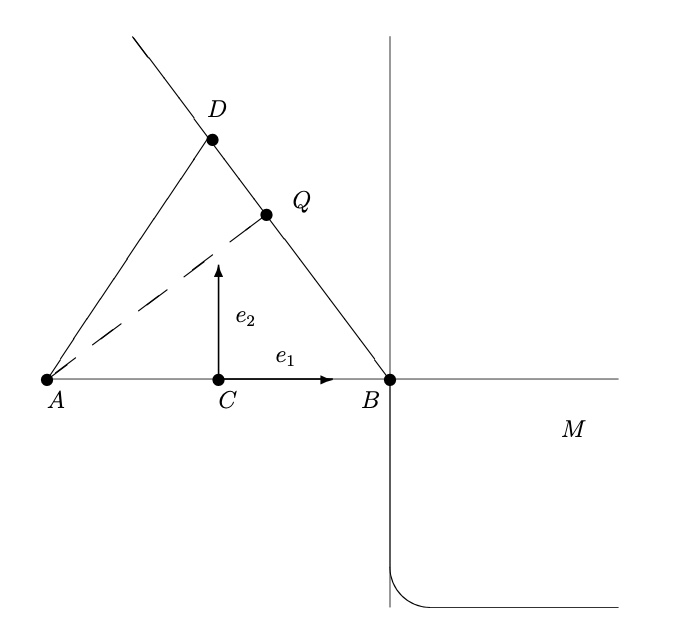
\includegraphics[width = 160mm]{2_1}
	\end{center}

	Если $Q \in [DB]$, то $Q \in M$ в силу выпуклости M. При этом $||AQ|| < ||AB||$, что противоречит выбору B.

	Проводя аналогичные рассуждения с N и функцией $-f$ получаем, что $(-f)|_N > \frac{r}{2}$, откуда $f|_N < 0$.
\end{Proof}

\begin{conseq}[]\label{cha:2/conseq:1}
	Если в доказательстве теоремы взять функцию $g = f - \frac{r}{2}$, то $g|_M \ge 0$ и $g|_N < 0$.
\end{conseq}

















